\documentclass[12pt,a4paper]{article}
\usepackage[top=25.4mm, bottom=25.4mm, left=19.1mm, right=19.1mm]{geometry}


\usepackage[latin2]{inputenc}
\usepackage{graphicx}
\graphicspath{ {./images/} }
\usepackage{ulem}
\usepackage{amsmath}
\usepackage[document]{ragged2e}

\setlength{\parindent}{4em}
\setlength{\parskip}{1em}
\usepackage{hyperref}

\usepackage{fancyhdr}
\pagestyle{fancy}
\fancyhf{}
\fancyhead[LO]{\textbf{\small IoT and Smart Analytics}\\
\text{\small A Program by IIITH and TalentSprint}}

\usepackage{xcolor}
\usepackage{lipsum}

\rhead{\begin{picture}(0,0) \put(-250,-2){
\includegraphics[width=9cm]{EXP_06_Images/ts-iisc-logo-pr.png}} \end{picture}}
\cfoot{\thepage}


\begin{document}
\begin{sloppypar}

\begin{center}

\textbf{\large \\EXPERIMENT 21 }\\[6pt]
\text{ Introduction to BLE on ESP32 }
\end{center}

\textbf{\large LEARNING OBJECTIVES:}\\[3pt]
At the end of this experiment, participants will be able to:\vspace{-6mm}\begin{enumerate}
 \setlength\itemsep{-0.3em}
\item Implement the basic BLE server using ESP32 \\
\item Observing BLE services and characteristics in the smartphone.
\end{enumerate}

\textbf{\large APPARATUS REQUIRED:}\\
\vspace{-3mm}
\begin{enumerate}
 \setlength\itemsep{-0.3em}
\item ESP32 Module-2pcs 
\item Micro USB cable-1pcs
\item Smartphone
\item Arduino IDE
\end{enumerate}

\begin{justify}
\textbf{\large THEORY}\\[3pt]
\textbf{Introduction}: Bluetooth Low Energy, BLE for short, is a power-conserving variant of Bluetooth. BLE's primary application is a short-distance transmission of small amounts of data (low bandwidth). Unlike Bluetooth that is always on, BLE remains in sleep mode constantly except for when a connection is initiated.\par
\noindent This makes it consume very low power. BLE consumes approximately 100x less power than Bluetooth (depending on the use case).\par
\noindent Due to its properties, BLE is suitable for applications that need to exchange small amounts of data periodically running on a coin cell. For example, BLE is of great use in healthcare, fitness, tracking, beacons, security, and home automation industries.\par
\noindent \textbf{BLE Server and Client:} With Bluetooth Low Energy, there are two types of devices: the server and the client. The ESP32 can act either as a client or as a server.
The server advertises its existence, so it can be found by other devices and contains the data that the client can read. The client scans the nearby devices, and when it finds the server it is looking for, it establishes a connection and listens for incoming data. This is called point-to-point communication.\par
\noindent \textbf{GATT: }GATT stands for Generic Attributes and it defines a hierarchical data structure that is exposed to connected BLE devices. This means that GATT defines the way that two BLE devices send and receive standard messages. Understanding this hierarchy is important because it will make it easier to understand how to use the BLE and write your applications.

\begin{center} 
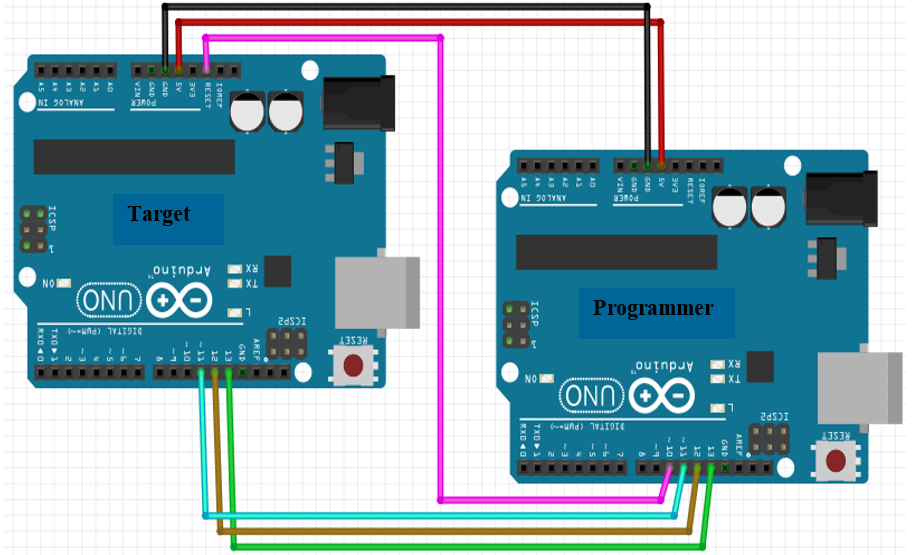
\includegraphics[scale=0.7]{EXP_21_Images/fig1.png}
\end{center}
\begin{center} {Figure 1. BLE Hierarchy}\end{center}

\noindent \textbf{BLE Service: }The top-level of the hierarchy is a profile, which is composed of one or more services. Usually, a BLE device contains more than one service.\par
\noindent Every service contains at least one characteristic, or can also reference other services. A service is simply a collection of information, like sensor readings, for example.\par
\noindent There are predefined services for several types of data defined by the SIG (Bluetooth Special Interest Group) viz. Battery Level, Blood Pressure, Heart Rate, Weight Scale, etc.

\noindent \textbf{BLE Characteristic: }The characteristic is always owned by a service, and it is where the actual data is contained in the hierarchy (value). The characteristic always has two attributes: characteristic declaration (that provides metadata about the data) and the characteristic value.\par
\noindent Additionally, the characteristic value can be followed by descriptors, which further expand on the metadata contained in the characteristic declaration.\par
\noindent The properties describe how the characteristic value can be interacted with. It contains the operations and procedures that can be used with the characteristic:

\begin{itemize}
 \setlength\itemsep{-0.3em}
 \item Broadcast
\item Read
\item Write without response
\item Write
\item Notify
\item Indicate
\item Authenticated Signed Writes
\item Extended Properties
\end{itemize}


\noindent \textbf{UUID: } Each service, characteristic, and descriptor have a UUID (Universally Unique Identifier). A UUID is a unique 128-bit (16 bytes) number.\par
\noindent There are shortened UUIDs for all types, services, and profiles specified in the
\underline{SIG (Bluetooth Special Interest Group)}.\par
\noindent But if your application needs its own UUID, you can generate it using this  \underline{UUID generator website}.\par
\noindent In summary, the UUID is used for uniquely identifying information. For example, it can identify a particular service provided by a Bluetooth device.\\[21pt]
\noindent \textbf{\large PROCEDURE}\\[6pt]
\textbf{A) Setting BLE Server in one ESP32 and Scanning with other.}
\vspace{-3mm}
\begin{enumerate}
\setlength\itemsep{-0.3em}
\item  Open your Arduino IDE and go to \textbf{ File $>$ Examples $>$ ESP32 BLE } Arduino and select the \textbf{ BLE\_server} example.

\item The following line of the code will define the name of your BLE server. Change it to whatever you would like to name your server.
\begin{center} \textcolor{blue}{ BLEDevice::init("Your server name");} \end {center} 

\item  Modify the following line of code in the example to the message that you wish to see on your smartphone.
\begin{center} 
\textcolor{blue}{$pCharacteristic->setValue("Hello World says Neil")$}
\end{center}

\item Upload this code to your ESP32 module. After uploading, we would have successfully created a BLE server. In the following steps, we will take a second ESP32 module which shall work as a scanner.

\item In your Arduino IDE, go to \textbf{File $>$ Examples $>$ ESP32 BLE Arduino} and select the \textbf{BLE\_scan} example.
\item Upload this code to the other ESP32 module.
\item Now, power on both devices and open the serial monitor for the ESP32 that contains code for scanning. The output should look something similar to the following figure-
\end{enumerate}

\begin{center} 
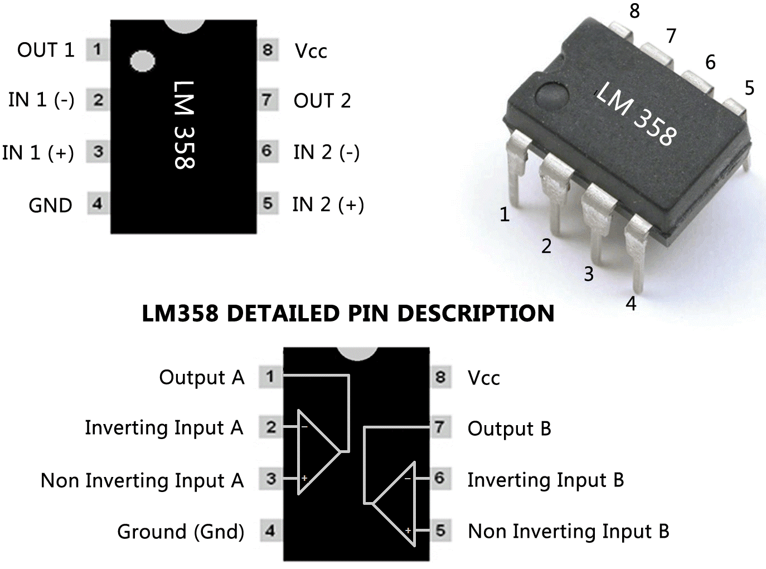
\includegraphics[scale=0.75]{EXP_21_Images/fig2.png}
\end{center}
\begin{center} {Figure 2. BLE scan output}\end{center}

\noindent \textbf{B) Scanning with other devices(e.g. mobile) having BLE support.}
\vspace{-3mm}
\begin{enumerate}
\setlength\itemsep{-0.3em}
\item Download the nRF Connect app. It is available for Android as well as iOS. 

\begin{center} 
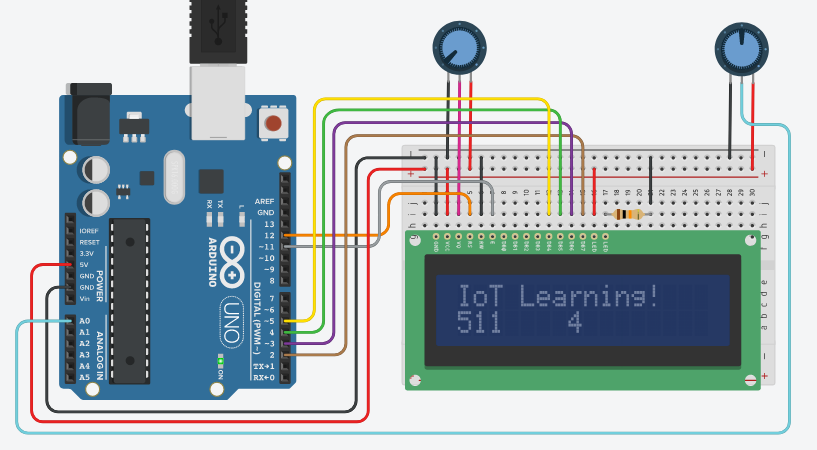
\includegraphics[scale=0.75]{EXP_21_Images/fig3.png}
\end{center}
\begin{center} {Figure 3. nRF Connect app installation}\end{center}

\item Open the app and enable Bluetooth and location. The further steps are fairly simple.
\item Press the scan button and connect to your BLE server.
\item You should be able to see the services and characteristics with the UUID defined in the code. The default message will also be displayed that is mentioned in the example code.
\begin{center} 
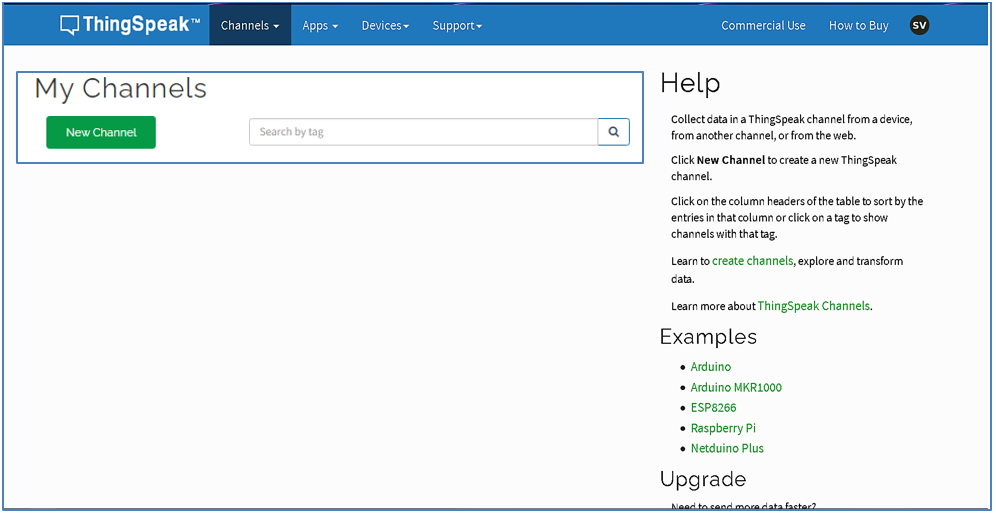
\includegraphics[scale=0.8]{EXP_21_Images/fig4.png}
\end{center}
\begin{center} {Figure 4. Message displayed on the app }\end{center}
\end{enumerate}



\textbf{\large REFERENCES:}
\vspace{-6mm}
\begin{enumerate}
\setlength\itemsep{-0.3em}
 \item  \href{https://www.arduino.cc/reference/en/libraries/esp32-ble-arduino/}{ESP32-BLE-Arduino}
\item   \href{https://randomnerdtutorials.com/esp32-bluetooth-low-energy-ble-arduino-ide/}{ESP32 BLE Arduino IDE}
\end{enumerate}
\end{justify}
\end{sloppypar}
\end{document}